% !TeX program = tectonic
% !TeX root = intro.tex
\documentclass[aspectratio=169,10pt]{beamer}

\usepackage[T1]{fontenc}
\renewcommand{\rmdefault}{ptm}
\renewcommand{\sfdefault}{phv}
\usefonttheme{professionalfonts}
\usepackage{amsmath,amssymb}
\usepackage{graphicx}
\usepackage{animate}
\usepackage{qrcode}
\usepackage{tikz}
\usetikzlibrary{arrows.meta,calc,fit,positioning}

\definecolor{Ink}{HTML}{17243A}
\definecolor{BrandBlue}{HTML}{1E90FF}
\colorlet{Navy}{BrandBlue}
\definecolor{Ice}{HTML}{E9EFF4}
\definecolor{Mist}{HTML}{F4F6F8}
\definecolor{Slate}{HTML}{64748B}
\definecolor{TerrainLight}{HTML}{DCE8E5}
\definecolor{TerrainMid}{HTML}{AFC8C4}
\definecolor{TerrainDark}{HTML}{769E9A}
\definecolor{Trail}{HTML}{D89A43}
\definecolor{TrailDark}{HTML}{9E6424}

\setbeamercolor{normal text}{fg=Ink,bg=white}
\setbeamercolor{structure}{fg=BrandBlue}
\setbeamercolor{frametitle}{fg=white,bg=BrandBlue}
\setbeamercolor{block title}{fg=white,bg=BrandBlue}
\setbeamercolor{block body}{fg=Ink,bg=BrandBlue!7!white}
\setbeamerfont{frametitle}{series=\bfseries,size=\large}
\setbeamertemplate{navigation symbols}{}
\setbeamertemplate{itemize item}{$\color{BrandBlue}\blacktriangleright$}
\setbeamertemplate{footline}{%
  \leavevmode%
  \hbox{%
    \begin{beamercolorbox}[wd=.075\paperwidth,ht=2.6ex,dp=1.1ex,center]{author in head/foot}%
      \raisebox{-0.65ex}[0pt][0pt]{
\includegraphics[height=4.2ex]{assets/logos/atari_lab.png}}%
    \end{beamercolorbox}%
    \begin{beamercolorbox}[wd=.785\paperwidth,ht=2.6ex,dp=1.1ex,leftskip=0.35em]{author in head/foot}%
      \color{Slate}\scriptsize Sebastian Sanokowski \textbar{} Research introduction
    \end{beamercolorbox}%
    \begin{beamercolorbox}[wd=.14\paperwidth,ht=2.6ex,dp=1.1ex,center]{date in head/foot}%
      \color{BrandBlue}\scriptsize\insertframenumber/\inserttotalframenumber
    \end{beamercolorbox}%
  }%
}

\newcommand{\frametumlogo}{%
  \begin{tikzpicture}[remember picture,overlay]
    \node[anchor=north east,fill=white,rounded corners=1.2pt,
          inner xsep=2.8pt,inner ysep=1.8pt]
      at ([xshift=-0.16cm,yshift=-0.10cm]current page.north east)
      {
\includegraphics[height=0.52cm]{assets/logos/tum_logo.png}};
  \end{tikzpicture}%
}

\newcommand{\plainlogos}{%
  \begin{tikzpicture}[remember picture,overlay]
    \node[anchor=north east,fill=white,rounded corners=1.2pt,
          inner xsep=2.8pt,inner ysep=1.8pt]
      at ([xshift=-0.16cm,yshift=-0.12cm]current page.north east)
      {
\includegraphics[height=0.62cm]{assets/logos/tum_logo.png}};
    \node[anchor=south west,fill=white,rounded corners=1.2pt,inner sep=2pt]
      at ([xshift=0.16cm,yshift=0.13cm]current page.south west)
      {
\includegraphics[height=0.82cm]{assets/logos/atari_lab.png}};
  \end{tikzpicture}%
}

% Compact robot arm: color, opacity, shoulder, elbow, wrist, tool, rotation.
\newcommand{\drawrobotarm}[7]{%
  \draw[white,line width=7pt,opacity=0.92]
    (#3) -- (#4) -- (#5) -- (#6);
  \draw[#1,line width=4pt,opacity=#2]
    (#3) -- (#4) -- (#5) -- (#6);
  \node[circle,draw=#1,fill=white,opacity=#2,line width=1.1pt,
        minimum size=6pt,inner sep=0pt] at (#3) {};
  \node[circle,draw=#1,fill=white,opacity=#2,line width=1.1pt,
        minimum size=6pt,inner sep=0pt] at (#4) {};
  \node[circle,draw=#1,fill=white,opacity=#2,line width=1.1pt,
        minimum size=6pt,inner sep=0pt] at (#5) {};
  \node[circle,draw=#1,fill=white,opacity=#2,line width=1.1pt,
        minimum size=6pt,inner sep=0pt] at (#6) {};
  \begin{scope}[shift={(#6)},rotate=#7,opacity=#2]
    \draw[#1,line width=2.2pt] (0,0)--(0.24,0);
    \draw[#1,line width=1.7pt]
      (0.24,-0.16)--(0.24,0.16)
      (0.24,0.16)--(0.51,0.09)
      (0.24,-0.16)--(0.51,-0.09);
  \end{scope}%
}

\newcommand{\drawrobotbase}[2]{%
  \path[fill=Slate!24,draw=Slate!62,rounded corners=1.5pt]
    ({#1-0.38},{#2-0.28}) rectangle ({#1+0.38},{#2});
  \path[fill=Slate!38,draw=Slate!68]
    ({#1-0.25},{#2}) -- ({#1+0.25},{#2})
    -- ({#1+0.17},{#2+0.34}) -- ({#1-0.17},{#2+0.34}) -- cycle;
}

\newcommand{\Tau}{\mathcal{T}}

\title{Sebastian Sanokowski}
\author{Sebastian Sanokowski}
\institute{Applied and Theoretical Aspects of Robot Intelligence Lab (ATARI)}
\date{}

\begin{document}

% 0:00--0:20. Opening slide: name, affiliation, and two research examples.
\begin{frame}[plain]
  \begin{tikzpicture}[remember picture,overlay]
    \fill[BrandBlue!5]
      ([xshift=9.15cm]current page.south west) rectangle (current page.north east);
    \path[fill=BrandBlue!10]
      ([xshift=9.15cm]current page.south west)
      -- (current page.south east) -- (current page.north east)
      -- ([xshift=12.05cm]current page.north west) -- cycle;
  \end{tikzpicture}
  \plainlogos

  \vspace{0.95cm}
  \begin{columns}[onlytextwidth]
    \column{0.56\textwidth}
      {\fontsize{27}{30}\selectfont\bfseries\color{BrandBlue}
        Sebastian Sanokowski}\par
      \vspace{0.16cm}
      {\large\bfseries\color{Ink}Postdoc}\par
      \vspace{0.07cm}
      {\normalsize\color{Ink}
        Applied and Theoretical Aspects of\\
        Robot Intelligence Lab (ATARI)}\par
      \vspace{0.46cm}
      {\large\bfseries Multimodal Diffusion Policies in RL}\par

    \column{0.40\textwidth}
      \centering
      {\scriptsize\bfseries\color{Ink}REAL-WORLD HUMANOID}\par
      \vspace{0.04cm}
      \animategraphics[autoplay,loop,poster=first,width=0.92\linewidth]
        {4}{assets/humanoid_motion_a/frame-}{0}{47}
      \vspace{0.13cm}

      {\scriptsize\bfseries\color{Ink}MULTIMODAL ROBOT POLICY}\par
      \vspace{0.04cm}
      \animategraphics[autoplay,loop,poster=last,height=1.95cm]
        {5}{assets/stackcube_overlay/frame-}{0}{22}
  \end{columns}
\end{frame}

% 0:20--0:50. Reuse the opening robotics illustration from the tutorial.
\begin{frame}{Robotics has many valid solutions}
  \centering
  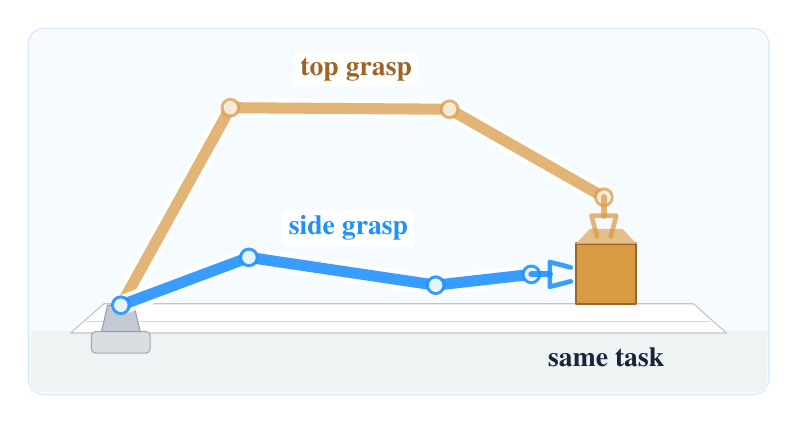
\begin{tikzpicture}[x=0.98cm,y=0.98cm,font=\small,
      line cap=round,line join=round]
    \path[fill=BrandBlue!4,draw=BrandBlue!20,rounded corners=6pt]
      (0,0) rectangle (9.6,4.75);
    \path[fill=TerrainLight!48!white]
      (0.03,0.03) rectangle (9.57,0.82);
    \path[fill=white,draw=Slate!42]
      (0.55,0.80) -- (9.05,0.80) -- (8.62,1.18) -- (0.98,1.18) -- cycle;
    \draw[Slate!28,line width=0.6pt] (0.76,0.95) -- (8.83,0.95);
    \drawrobotbase{1.20}{0.82}
    \path[fill=Trail,draw=TrailDark,line width=0.8pt]
      (7.10,1.18) rectangle (7.88,1.96);
    \path[fill=Trail!64!white]
      (7.10,1.96) -- (7.88,1.96) -- (7.70,2.15) -- (7.28,2.15) -- cycle;
    \draw[TrailDark!60,line width=0.6pt] (7.10,1.96) -- (7.88,1.96);
    \node[text=Ink,font=\bfseries] at (7.49,0.48) {same task};

    \drawrobotarm{Trail}{0.72}{1.20,1.16}{2.62,3.72}{5.46,3.70}{7.46,2.56}{-90}
    \node[text=TrailDark,font=\bfseries,fill=white,inner sep=2pt]
      at (4.25,4.22) {top grasp};
    \drawrobotarm{BrandBlue}{0.88}{1.20,1.16}{2.86,1.78}{5.28,1.42}{6.52,1.56}{0}
    \node[text=BrandBlue,font=\bfseries,fill=white,inner sep=2pt]
      at (4.15,2.16) {side grasp};
  \end{tikzpicture}
  \vspace{0.15cm}

  {\large\bfseries A trained policy should represent every valid solution.}
  \frametumlogo
\end{frame}

% 0:50--1:20. Robotics-grounded reasons to retain multiple solution modes.
\begin{frame}{What multimodality buys us}
  \begin{columns}[T,onlytextwidth]
    \column{0.32\textwidth}
      \centering
      {\bfseries\color{Ink}Better exploration}\par\vspace{0.12cm}
      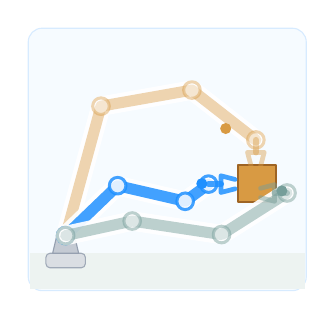
\begin{tikzpicture}[x=0.66cm,y=0.66cm,line cap=round,line join=round]
        \path[fill=BrandBlue!4,draw=Navy!18,rounded corners=5pt]
          (0,0) rectangle (5.35,5.05);
        \path[fill=TerrainLight!52!white]
          (0.03,0.03) rectangle (5.32,0.72);
        \drawrobotbase{0.72}{0.72}
        \path[fill=Trail,draw=TrailDark,line width=0.7pt]
          (4.04,1.70) rectangle (4.76,2.42);
        \drawrobotarm{Trail}{0.42}{0.72,1.06}{1.40,3.55}{3.15,3.86}{4.38,2.90}{-90}
        \drawrobotarm{BrandBlue}{0.84}{0.72,1.06}{1.72,2.02}{3.02,1.72}{3.47,2.05}{0}
        \drawrobotarm{TerrainDark}{0.48}{0.72,1.06}{2.00,1.34}{3.72,1.08}{4.98,1.88}{180}
        \foreach \x/\y/\c in {3.80/3.12/Trail,3.34/2.06/BrandBlue,
          4.88/1.92/TerrainDark}{\fill[\c] (\x,\y) circle (2.0pt);}
      \end{tikzpicture}

    \column{0.32\textwidth}
      \centering
      {\bfseries\color{Ink}Better adaptability}\par\vspace{0.12cm}
      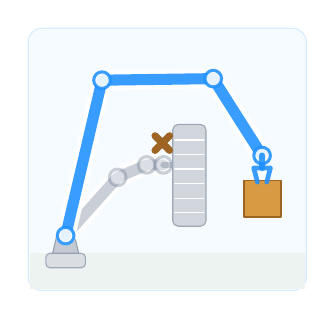
\begin{tikzpicture}[x=0.66cm,y=0.66cm,line cap=round,line join=round]
        \path[fill=BrandBlue!4,draw=Navy!18,rounded corners=5pt]
          (0,0) rectangle (5.35,5.05);
        \path[fill=TerrainLight!52!white]
          (0.03,0.03) rectangle (5.32,0.72);
        \drawrobotbase{0.72}{0.72}
        \path[fill=Trail,draw=TrailDark,line width=0.7pt]
          (4.16,1.42) rectangle (4.86,2.12);
        \drawrobotarm{Slate}{0.34}{0.72,1.06}{1.72,2.18}{2.28,2.42}{2.60,2.42}{0}
        \path[fill=Slate!30,draw=Slate!64,rounded corners=2pt]
          (2.78,1.24) rectangle (3.42,3.20);
        \foreach \y in {1.50,1.78,2.06,2.34,2.62,2.90}{
          \draw[white!78,line width=0.45pt] (2.82,\y) -- (3.38,\y);
        }
        \draw[TrailDark,line width=2.6pt]
          (2.44,2.70) -- (2.72,2.98)
          (2.72,2.70) -- (2.44,2.98);
        \drawrobotarm{BrandBlue}{0.88}{0.72,1.06}{1.42,4.05}{3.56,4.08}{4.50,2.60}{-90}
      \end{tikzpicture}

    \column{0.32\textwidth}
      \centering
      {\bfseries\color{Ink}Better world model}\par\vspace{0.12cm}
      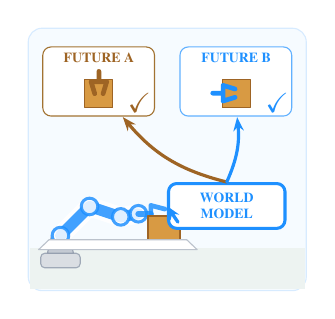
\begin{tikzpicture}[x=0.66cm,y=0.66cm,line cap=round,line join=round]
        \path[fill=BrandBlue!4,draw=Navy!18,rounded corners=5pt]
          (0,0) rectangle (5.35,5.05);
        \path[fill=TerrainLight!52!white]
          (0.03,0.03) rectangle (5.32,0.82);
        \drawrobotbase{0.62}{0.72}
        \drawrobotarm{BrandBlue}{0.84}{0.62,1.06}{1.18,1.62}{1.78,1.42}{2.12,1.48}{0}
        \path[fill=Trail,draw=TrailDark,line width=0.7pt]
          (2.30,0.82) rectangle (2.92,1.44);
        \path[fill=white,draw=Slate!44]
          (0.20,0.79) -- (3.25,0.79) -- (3.05,0.98) -- (0.40,0.98) -- cycle;
        \node[draw=BrandBlue,fill=white,rounded corners=3pt,line width=1.1pt,
              text=BrandBlue,font=\bfseries\tiny,minimum width=1.48cm,
              minimum height=0.50cm,align=center] (model) at (3.82,1.63)
          {WORLD\\MODEL};
        \draw[-{Stealth[length=5pt]},BrandBlue,line width=1.2pt]
          (2.88,1.32) -- (model.west);
        \path[fill=white,draw=Trail!75!black,rounded corners=3pt]
          (0.28,3.36) rectangle (2.43,4.69);
        \path[fill=white,draw=BrandBlue!70,rounded corners=3pt]
          (2.92,3.36) rectangle (5.07,4.69);
        \node[text=TrailDark,font=\bfseries\tiny] at (1.36,4.48) {FUTURE A};
        \node[text=BrandBlue,font=\bfseries\tiny] at (4.00,4.48) {FUTURE B};
        \path[fill=Trail,draw=TrailDark] (1.09,3.52) rectangle (1.63,4.06);
        \path[fill=Trail,draw=TrailDark] (3.73,3.52) rectangle (4.27,4.06);
        \begin{scope}[shift={(1.36,4.22)},rotate=-90]
          \draw[TrailDark,line width=1.7pt]
            (0,0)--(0.20,0) (0.20,-0.15)--(0.20,0.15)
            (0.20,0.15)--(0.43,0.08) (0.20,-0.15)--(0.43,-0.08);
        \end{scope}
        \begin{scope}[shift={(3.55,3.80)}]
          \draw[BrandBlue,line width=1.7pt]
            (0,0)--(0.20,0) (0.20,-0.15)--(0.20,0.15)
            (0.20,0.15)--(0.43,0.08) (0.20,-0.15)--(0.43,-0.08);
        \end{scope}
        \node[text=TrailDark,font=\bfseries] at (2.14,3.62) {$\checkmark$};
        \node[text=BrandBlue,font=\bfseries] at (4.79,3.62) {$\checkmark$};
        \draw[-{Stealth[length=5pt]},TrailDark,line width=1.15pt]
          (model.north) to[bend left=18] (1.82,3.34);
        \draw[-{Stealth[length=5pt]},BrandBlue,line width=1.15pt]
          (model.north) to[bend right=15] (4.02,3.34);
      \end{tikzpicture}
  \end{columns}
  \frametumlogo
\end{frame}

% 1:20--1:50. Diffusion samplers replace demonstrations with an objective.
\begin{frame}{Diffusion samplers learn from a cost---not demonstrations}
  \centering
  \vspace{0.02cm}
  {\large
    $C(x)$\quad$\Longrightarrow$\quad
    $p_{\Tau}(x)\propto \exp\!\left(-C(x)/\Tau\right)$}
  \vspace{0.12cm}

  \animategraphics[autoplay,loop,poster=last,width=0.96\linewidth]
    {4}{assets/diffusion_transport/frame-}{0}{47}
  \vspace{0.08cm}

  {\large\bfseries Noise $\longrightarrow$ many low-cost solutions}
  \frametumlogo
\end{frame}

% 1:50--2:30. The augmented MDP exposes local denoising transitions to RL.
\begin{frame}{DA-MDPs turn denoising into RL steps}
  \centering
  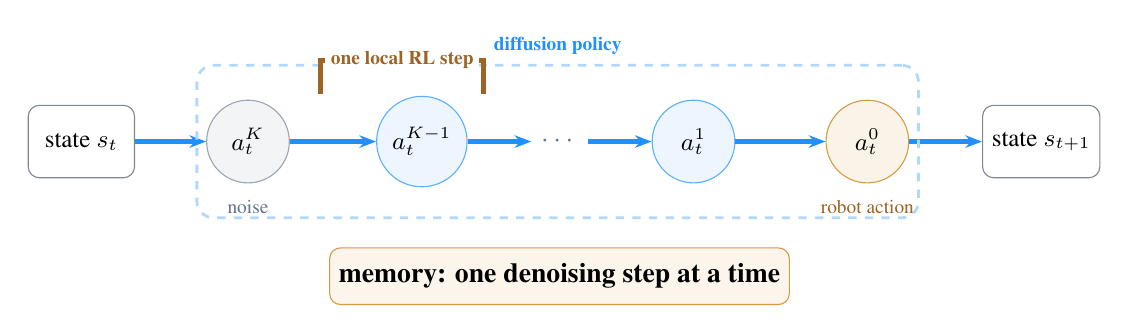
\begin{tikzpicture}[x=0.92cm,y=1cm,font=\small,
      flow/.style={-{Stealth[length=6pt]},BrandBlue,line width=1.5pt},
      state/.style={draw=Ink!55,fill=white,rounded corners=4pt,
                    minimum width=1.35cm,minimum height=0.92cm},
      action/.style={circle,draw=BrandBlue!72,fill=BrandBlue!8,
                     minimum size=1.05cm}]
    \node[state] (s) at (0.75,2.35) {state $s_t$};
    \node[action,draw=Slate!65,fill=Slate!8] (ak) at (3.05,2.35) {$a_t^K$};
    \node[action] (akm) at (5.45,2.35) {$a_t^{K-1}$};
    \node[text=Slate,font=\bfseries] (dots) at (7.35,2.35) {$\cdots$};
    \node[action] (aone) at (9.20,2.35) {$a_t^1$};
    \node[action,draw=Trail,fill=Trail!12] (azero) at (11.60,2.35) {$a_t^0$};
    \node[state] (sp) at (14.00,2.35) {state $s_{t+1}$};
    \draw[flow] (s)--(ak);
    \draw[flow] (ak)--(akm);
    \draw[flow] (akm)--(dots);
    \draw[flow] (dots)--(aone);
    \draw[flow] (aone)--(azero);
    \draw[flow] (azero)--(sp);
    \node[text=Slate,font=\scriptsize] at (3.05,1.52) {noise};
    \node[text=TrailDark,font=\scriptsize] at (11.60,1.52) {robot action};
    \node[draw=BrandBlue!35,rounded corners=6pt,dashed,line width=1pt,
          fit=(ak)(akm)(dots)(aone)(azero),inner ysep=11pt,
          label={[text=BrandBlue,font=\bfseries\scriptsize]above:
            diffusion policy}] {};
    \draw[TrailDark,line width=1.8pt]
      (4.05,2.96) -- (4.05,3.38) -- (6.30,3.38) -- (6.30,2.96);
    \node[text=TrailDark,font=\bfseries\scriptsize,fill=white,inner sep=2pt]
      at (5.18,3.38) {one local RL step};
    \node[draw=Trail,fill=Trail!10,rounded corners=4pt,
          font=\bfseries,minimum width=5.0cm,minimum height=0.72cm]
      at (7.35,0.64) {memory: one denoising step at a time};
  \end{tikzpicture}
  \vspace{0.10cm}

  \begin{columns}[T,onlytextwidth]
    \column{0.81\textwidth}
      \centering
      {\small\bfseries Any MaxEnt RL method}\par
      \vspace{0.08cm}
      \begin{columns}[onlytextwidth]
        \column{0.32\textwidth}\centering
          \colorbox{BrandBlue!8}{\strut PPO $\rightarrow$ \textbf{DA:PPO}}
        \column{0.34\textwidth}\centering
          \colorbox{BrandBlue!8}{\strut REPPO $\rightarrow$ \textbf{DA:REPPO}}
        \column{0.32\textwidth}\centering
          \colorbox{BrandBlue!8}{\strut WPO $\rightarrow$ \textbf{DA:WPO}}
      \end{columns}
      \vspace{0.11cm}

      {\tiny
        \href{https://arxiv.org/abs/2512.02019}
          {\textcolor{BrandBlue}{Sanokowski \& Patil (2026),
          \emph{Diffusion-Augmented MDPs}, arXiv:2512.02019.}}}
    \column{0.17\textwidth}
      \centering
      \href{https://arxiv.org/abs/2512.02019}{%
        \qrcode[height=1.52cm]{https://arxiv.org/abs/2512.02019}}
      \par\vspace{0.03cm}
      {\tiny\bfseries\color{BrandBlue}DA-MDP paper}
  \end{columns}
  \frametumlogo
\end{frame}

% 2:30--2:55. First application: both modes of the symmetric StackCube task.
\begin{frame}{DA:REPPO represents both StackCube solutions}
  \centering
  \animategraphics[autoplay,loop,poster=last,height=0.68\textheight]
    {5}{assets/stackcube_overlay/frame-}{0}{22}
  \vspace{0.08cm}

  {\large\bfseries One task. Two stacking orders. One policy.}
  \frametumlogo
\end{frame}

% 2:55--4:15. Data-only training, diffusion RL, and real-world transfer.
\begin{frame}{Nine diffusion-generated pickup motions---one scene}
  \begin{columns}[T,onlytextwidth]
    \column{0.32\textwidth}
      \centering
      \begin{minipage}[c][3.50cm][c]{\linewidth}
        \centering
        \animategraphics[autoplay,loop,poster=25,width=\linewidth,
            trim=240 0 170 120,clip]
          {5}{assets/humanoid_sim_pretrained_gallery/frame-}{0}{59}
      \end{minipage}\par
      \vspace{0.16cm}
      {\small\bfseries Training on data only}\par
      \vspace{0.07cm}
      {\scriptsize\color{Slate}5/9 pickups completed}
    \column{0.32\textwidth}
      \centering
      \begin{minipage}[c][3.50cm][c]{\linewidth}
        \centering
        \animategraphics[autoplay,loop,poster=25,width=\linewidth,
            trim=240 0 170 120,clip]
          {5}{assets/humanoid_sim_gallery/frame-}{0}{49}
      \end{minipage}\par
      \vspace{0.16cm}
      {\small\bfseries Diffusion RL fine-tuning}\par
      \vspace{0.07cm}
      {\scriptsize\color{Slate}9/9 pickups completed}
    \column{0.32\textwidth}
      \centering
      \begin{minipage}[c][3.50cm][c]{\linewidth}
        \centering
        \begin{animateinline}[autoplay,loop,poster=25]{4}
          \multiframe{48}{i=0+1}{%
            \includegraphics[width=\linewidth,trim=70 0 70 0,clip]
              {assets/humanoid_motion_a/frame-\i.jpg}%
          }
          \newframe
          \multiframe{40}{i=0+1}{%
            \includegraphics[width=\linewidth,trim=70 0 70 0,clip]
              {assets/humanoid_motion_b/frame-\i.jpg}%
          }
        \end{animateinline}
      \end{minipage}\par
      \vspace{0.16cm}
      {\small\bfseries Transfer to the real world}\par
      \vspace{0.07cm}
      {\scriptsize\color{Slate}Two motions, played consecutively}
  \end{columns}
  \frametumlogo
\end{frame}

% 4:15--4:50. Transition directly from this slide to main.pdf.
\begin{frame}{Tutorial: from variational inference to DA-MDPs}
  \small
  \begin{center}
    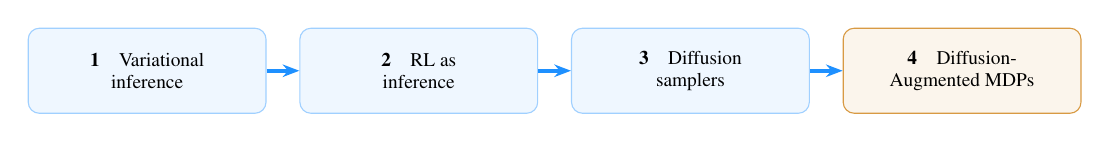
\begin{tikzpicture}[x=1cm,y=1cm,font=\scriptsize,
        lesson/.style={draw=BrandBlue!42,fill=BrandBlue!7,rounded corners=4pt,
                       align=center,minimum width=3.02cm,minimum height=1.08cm},
        flow/.style={-{Stealth[length=6pt]},BrandBlue,line width=1.35pt}]
      \node[lesson] (l1) at (1.55,0) {\textbf{1}\quad Variational\\inference};
      \node[lesson] (l2) at (5.00,0) {\textbf{2}\quad RL as\\inference};
      \node[lesson] (l3) at (8.45,0) {\textbf{3}\quad Diffusion\\samplers};
      \node[lesson,draw=Trail,fill=Trail!10] (l4) at (11.90,0)
        {\textbf{4}\quad Diffusion-\\Augmented MDPs};
      \draw[flow] (l1)--(l2);
      \draw[flow] (l2)--(l3);
      \draw[flow] (l3)--(l4);
    \end{tikzpicture}
  \end{center}
  \vspace{0.20cm}

  \begin{columns}[T,onlytextwidth]
    \column{0.79\textwidth}
      \begin{block}{Before the tutorial: install the course environment}
        \ttfamily\small
        git clone https://github.com/sanokows/SummerSchool.git\\
        cd SummerSchool\\
        uv sync --locked\\
        uv run jupyter lab
      \end{block}
      \vspace{0.06cm}

      \centering
      \href{https://github.com/sanokows/SummerSchool}
        {\textcolor{BrandBlue}{\textbf{github.com/sanokows/SummerSchool}}}
    \column{0.18\textwidth}
      \centering
      \href{https://github.com/sanokows/SummerSchool}{%
        \qrcode[height=2.08cm]{https://github.com/sanokows/SummerSchool}}
      \par\vspace{0.05cm}
      {\scriptsize\bfseries\color{BrandBlue}Tutorial repository}
  \end{columns}
  \frametumlogo
\end{frame}

% 4:50--5:00. Static closing slide.
\begin{frame}[plain]
  \begin{tikzpicture}[remember picture,overlay]
    \fill[BrandBlue] (current page.south west) rectangle (current page.north east);
    \path[fill=white,fill opacity=0.08]
      (current page.south west) -- (current page.north west)
      -- ([xshift=5.4cm]current page.north west)
      -- ([xshift=8.3cm]current page.south west) -- cycle;
    \node[align=center,text=white] at (current page.center)
      {{\bfseries\fontsize{30}{34}\selectfont Thank you for your attention}\\[0.34cm]
       {\large Sebastian Sanokowski}\\[0.12cm]
       {\normalsize Applied and Theoretical Aspects of Robot Intelligence Lab}\\[0.28cm]
       {\small\href{https://github.com/sanokows/SummerSchool}
         {github.com/sanokows/SummerSchool}}};
  \end{tikzpicture}
  \plainlogos
\end{frame}

\end{document}
